% vim: ts=2:sw=2:tw=80:et

\begin{figure}[hb]
  \centerline{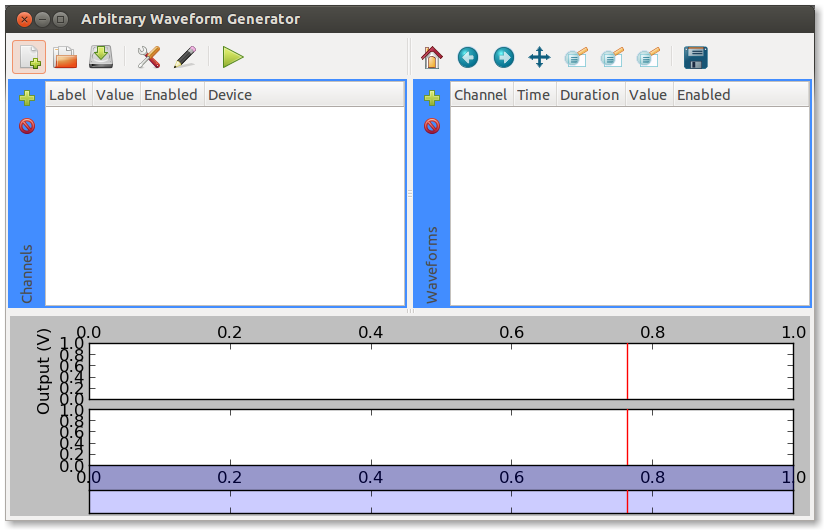
\includegraphics[width=\textwidth]{figures/main-empty}}
  \caption{Main window is empty upon startup}
  \label{fig:quick:main-empty}
\end{figure}



\begin{enumerate}
  \item Configure Devices

    \begin{figure}[ht]
      \centerline{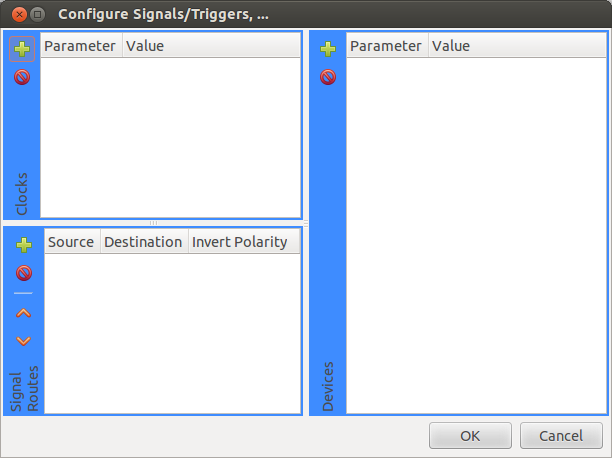
\includegraphics[width=.5\textwidth]{figures/configure-empty}}
      \caption{Configuration window is empty upon startup}
      \label{fig:quick:configure-empty}
    \end{figure}

    \begin{enumerate}
      \item Define Clocks

      \begin{figure}[ht]
        \centerline{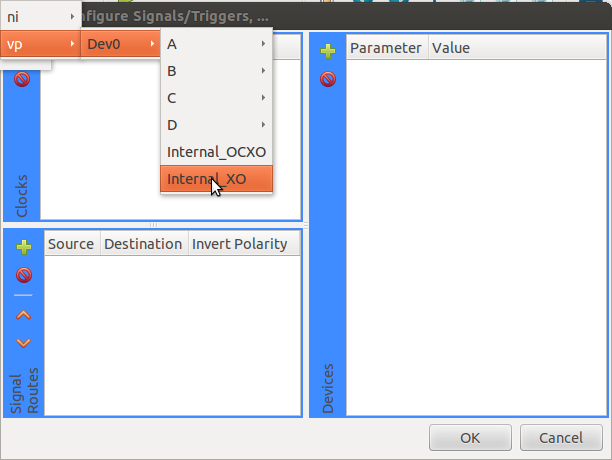
\includegraphics[width=.5\textwidth]{figures/configure-add-clock-vp-XO}}
        \caption{Configuration window while adding a Viewpoint internal crystal
        oscillator for use as a clock}
        \label{fig:quick:configure-add-clock-vp-XO}
      \end{figure}

      \begin{figure}[ht]
        \centerline{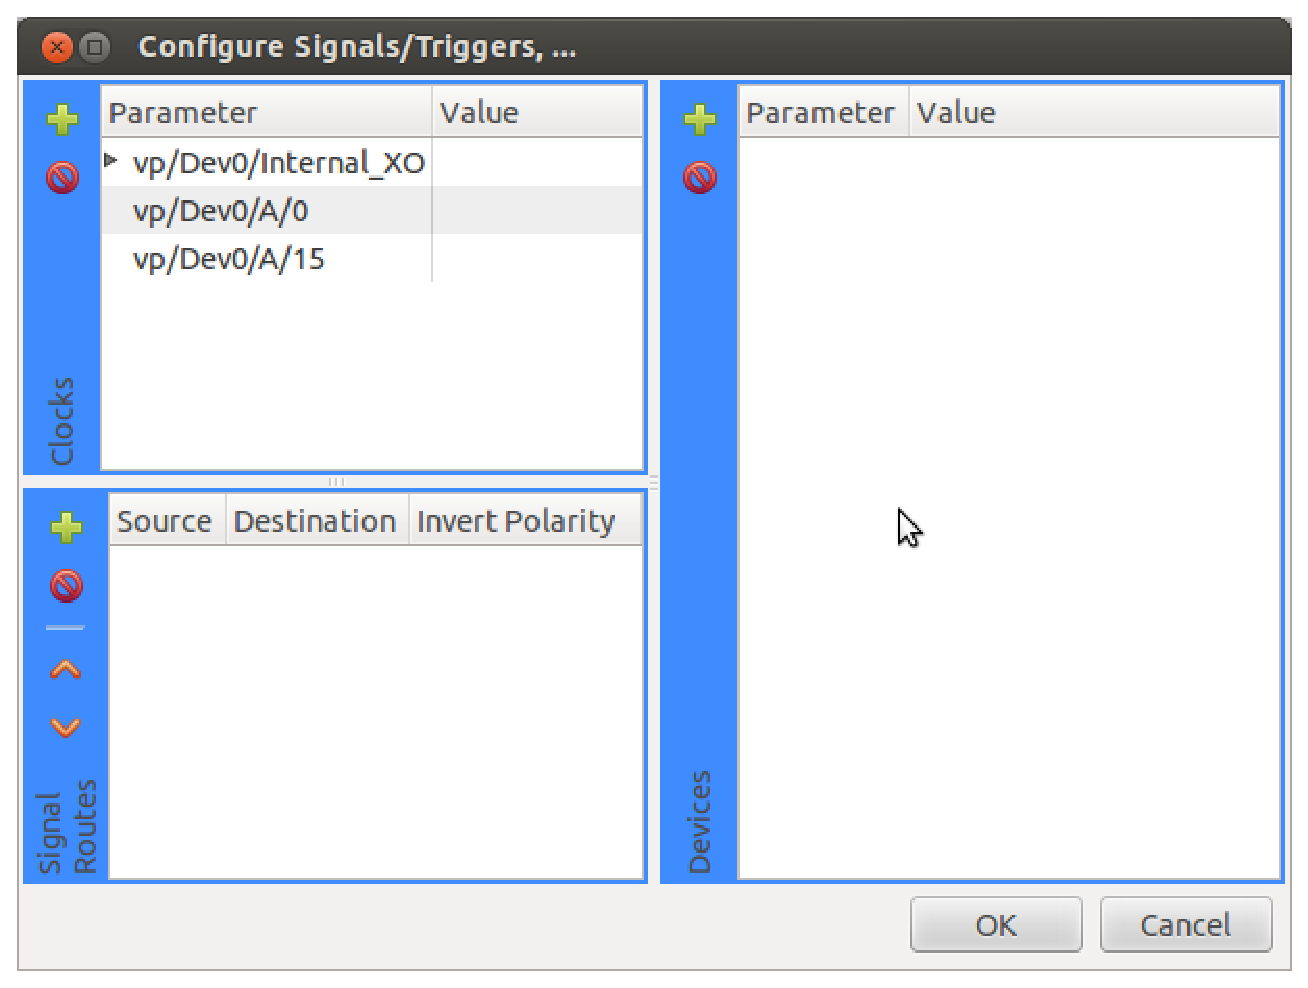
\includegraphics[width=.5\textwidth]{figures/configure-clocks-added}}
        \caption{Configuration window after having added various possible clocks}
        \label{fig:quick:configure-clocks-added}
      \end{figure}

      \item Define Signal Routes

      \begin{figure}[ht]
        \centerline{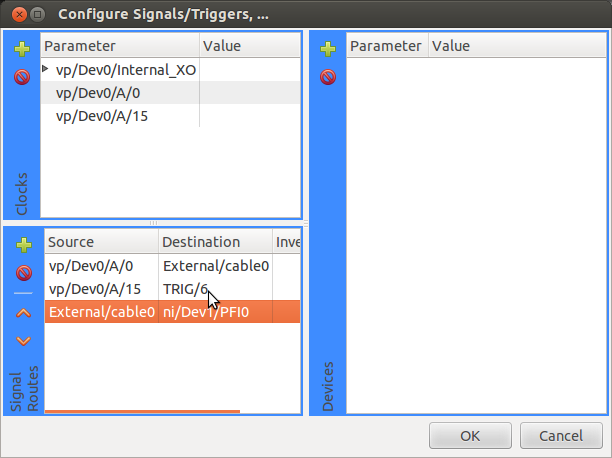
\includegraphics[width=.5\textwidth]{figures/configure-routes-added}}
        \caption{Configuration window after defining signal routes for clocks}
        \label{fig:quick:configure-routes-added}
      \end{figure}

      \item Define Clock Sources for Devices

      \begin{figure}[ht]
        \centerline{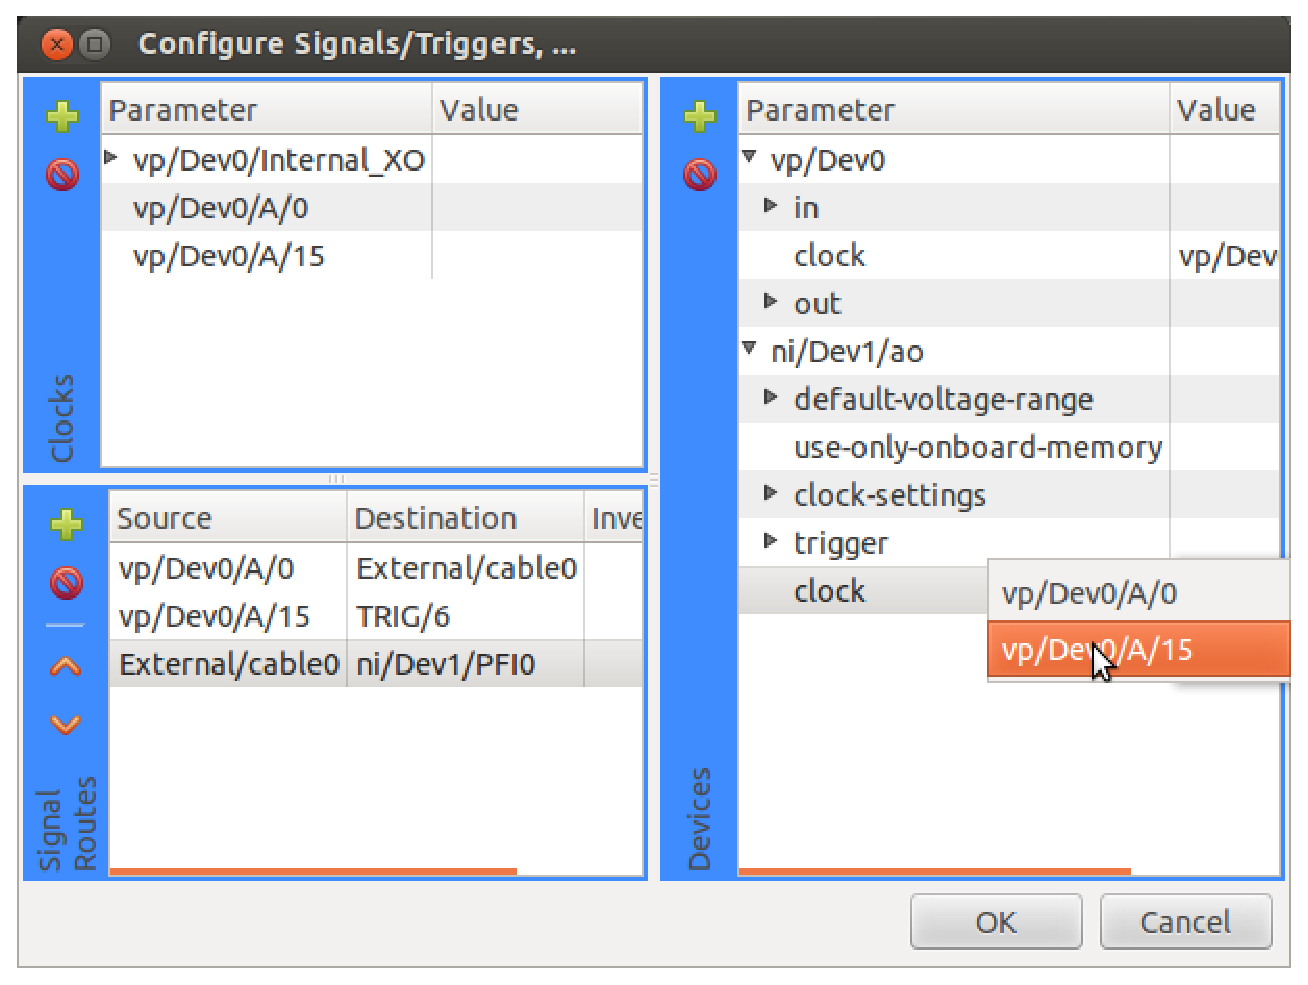
\includegraphics[width=.5\textwidth]{figures/configure-devices-set-clocks}}
        \caption{Configuration window after assigning appropriate clocks to
        devices}
        \label{fig:quick:configure-devices-set-clocks}
      \end{figure}

    \end{enumerate}
  \item Configure Channels
    \begin{enumerate}
      \item Channel Name
        The channel name should be used to very briefly describe the use of the
        particular physical output channel.  For example, for a digital output
        being used to trigger a camera, an appropriate channel name would be
        \textbf{Camera Trigger}.  \textbf{Channel Name} \textit{must} be unique with respect
        to all other enabled channels.
      \item Specifying Device
        The channel device selection describes the underlying hardware device
        and channel on that device that will be bound as the given
        \textbf{Channel Name}.  At most one channel should be bound to an
        underlying hardware output channel for all enabled channels.

        \begin{figure}[ht]
          \centerline{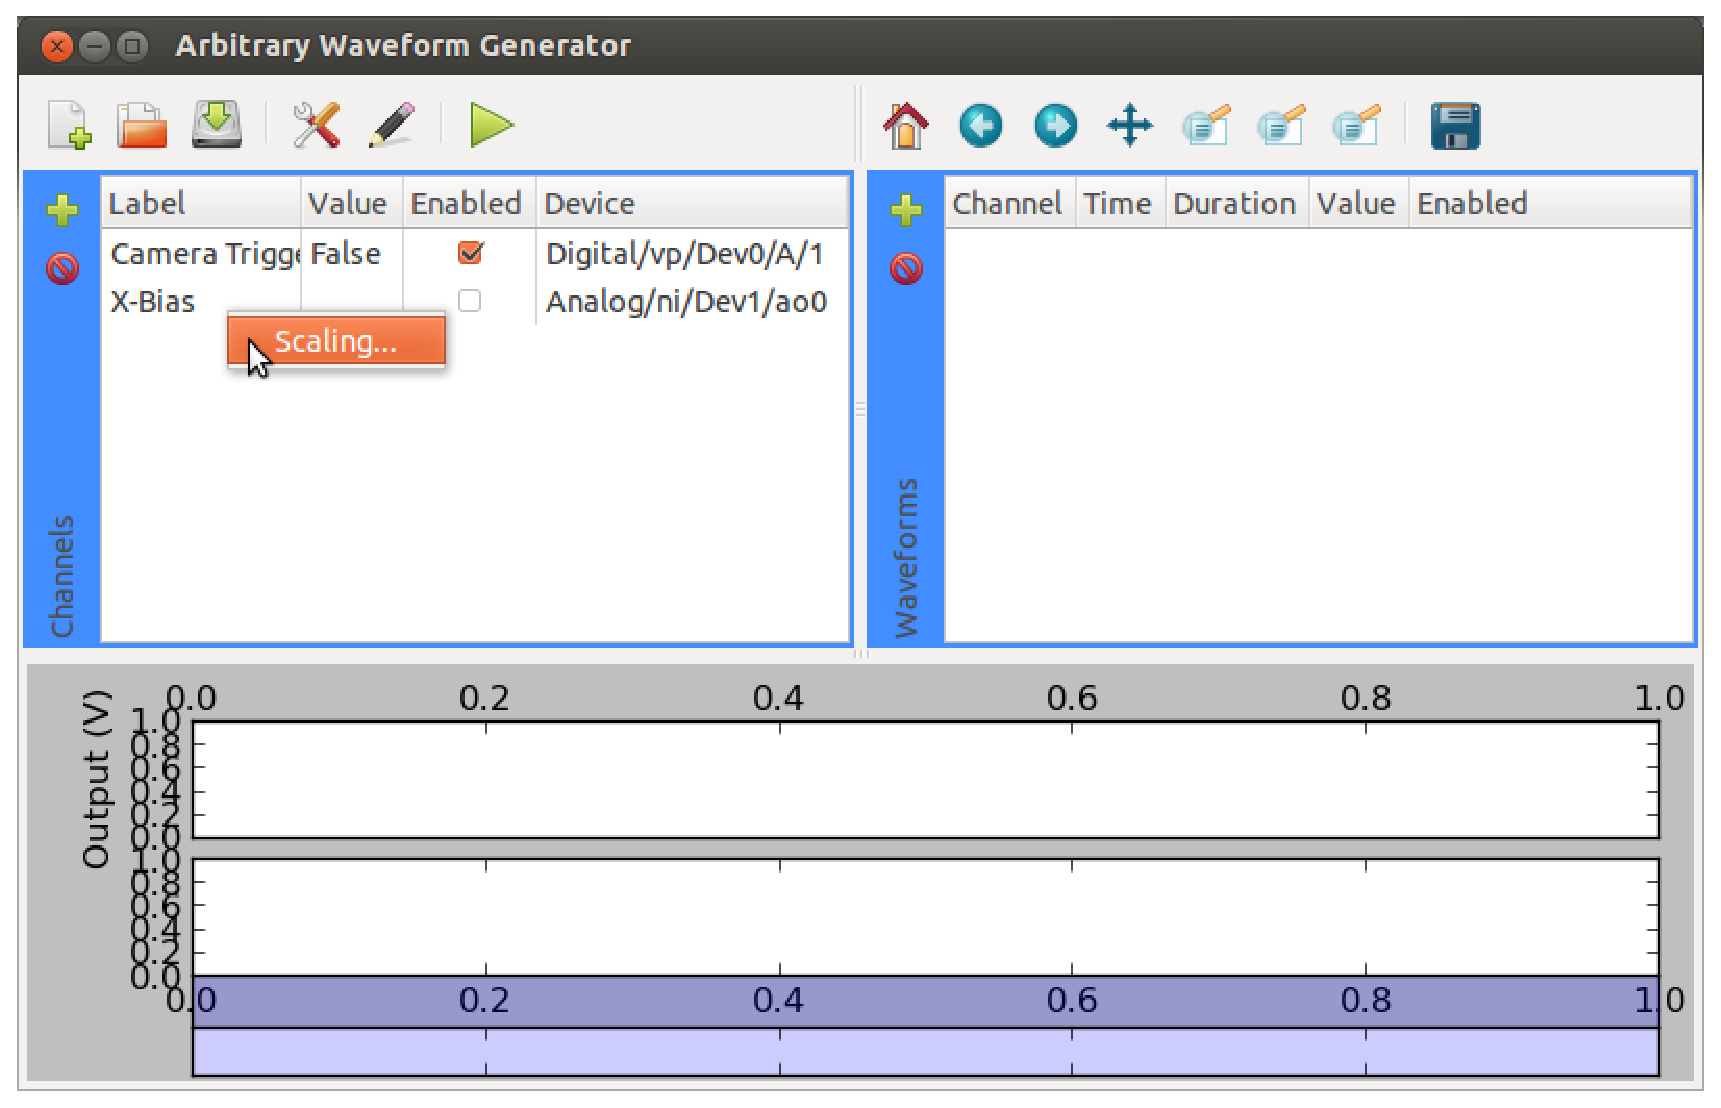
\includegraphics[width=.5\textwidth]{figures/channels-select-scaling}}
          \caption{Having added some channels, right click an analog channel to
          specify scaling/calibration.}
          \label{fig:quick:channels-select-scaling}
        \end{figure}


      \item Defining Scaling and Units

        \begin{figure}[ht]
          \centerline{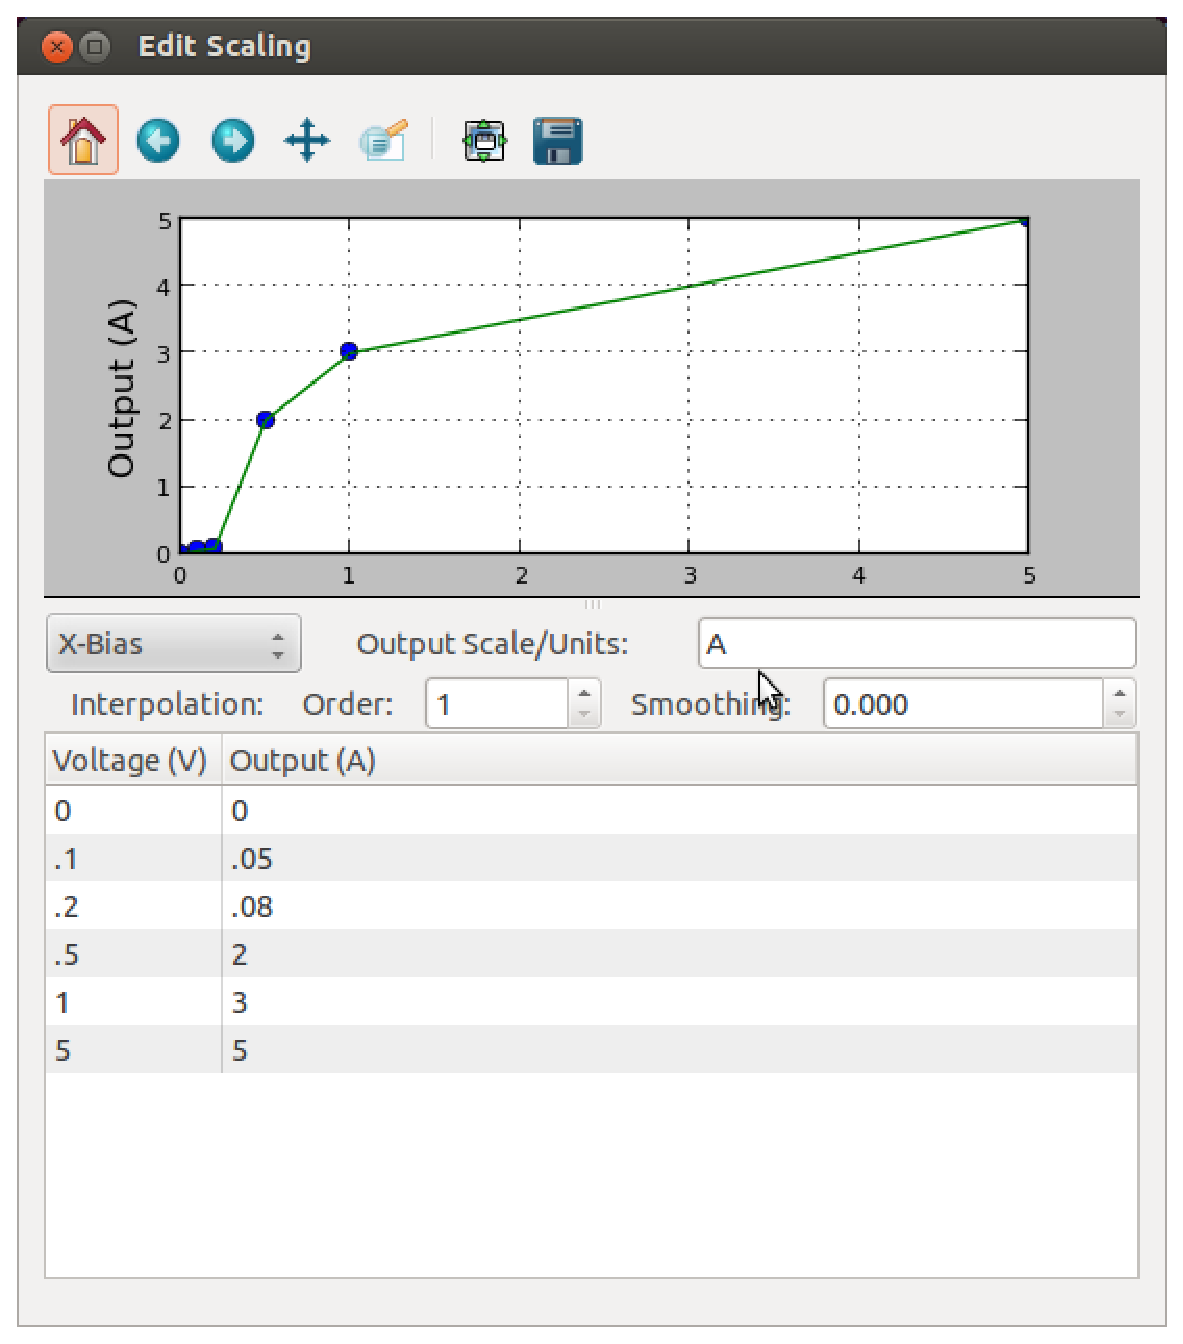
\includegraphics[width=.5\textwidth]{figures/scaling}}
          \caption{Specify the units and scaling or calibration on analog
          channels.}
          \label{fig:quick:scaling}
        \end{figure}

      \item Static Values
      \item Enabling
    \end{enumerate}
  \item Build Waveforms
    \begin{enumerate}
      \item Define Groups and Waveform Elements

        \begin{figure}[ht]
          \centerline{a)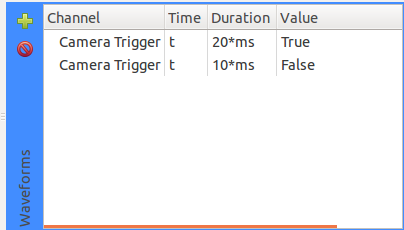
\includegraphics[width=.5\textwidth]{figures/waveform-0}}
          \centerline{b)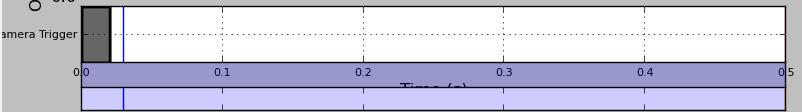
\includegraphics[width=.8\textwidth]{figures/plot-0}}
          \caption{a) Add some simple waveform elements. b) Plot of simple
          waveform elements.}
          \label{fig:quick:waveform-0}
        \end{figure}

        \begin{figure}[ht]
          \centerline{a)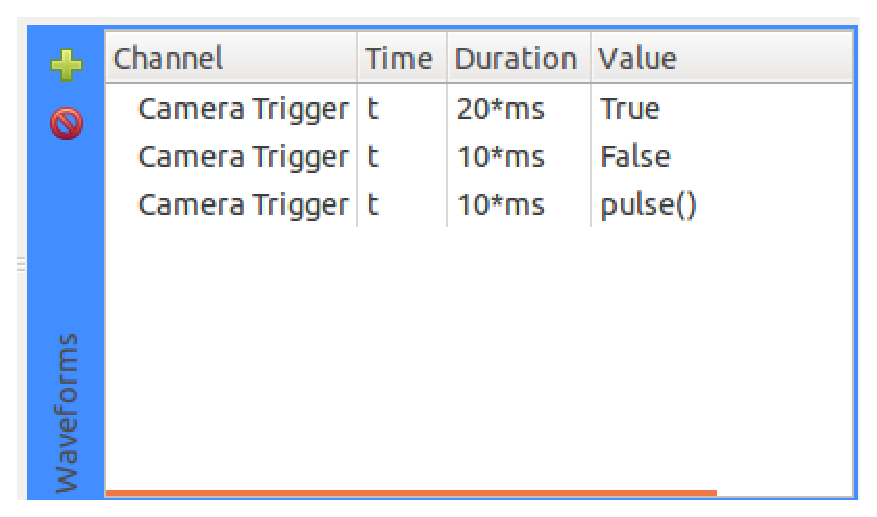
\includegraphics[width=.5\textwidth]{figures/waveform-1}}
          \centerline{b)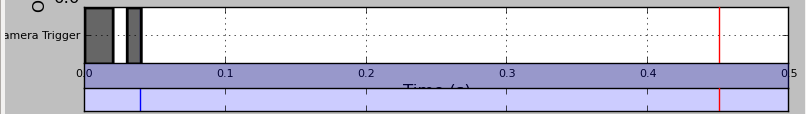
\includegraphics[width=.8\textwidth]{figures/plot-1}}
          \caption{a) Add some simple waveform elements. b) Plot of simple
          waveform elements.}
          \label{fig:quick:waveform-1}
        \end{figure}

        \begin{figure}[ht]
          \centerline{a)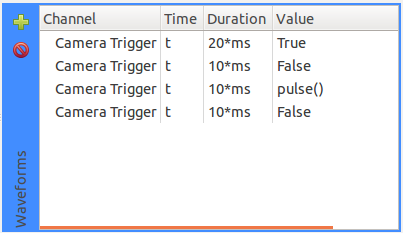
\includegraphics[width=.5\textwidth]{figures/waveform-2}}
          \centerline{b)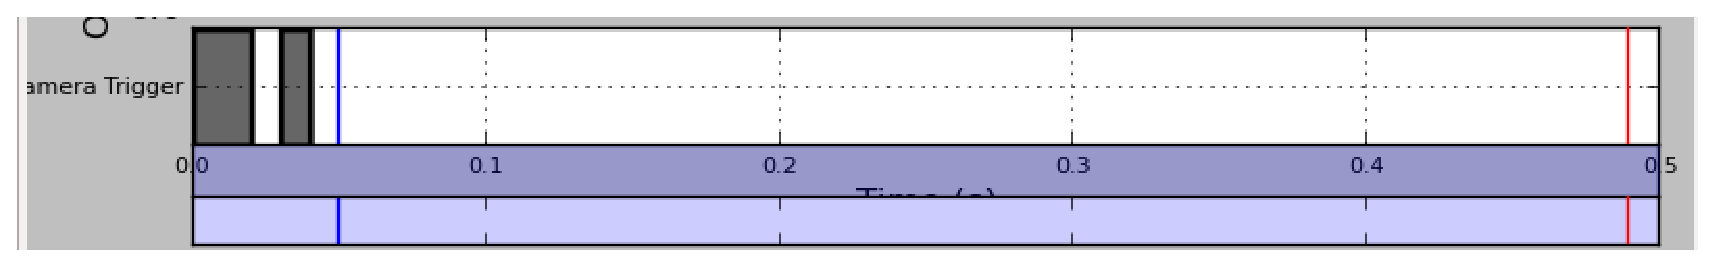
\includegraphics[width=.8\textwidth]{figures/plot-2}}
          \caption{a) Add some simple waveform elements. b) Plot of simple
          waveform elements.}
          \label{fig:quick:waveform-2}
        \end{figure}

        \begin{figure}[ht]
          \centerline{a)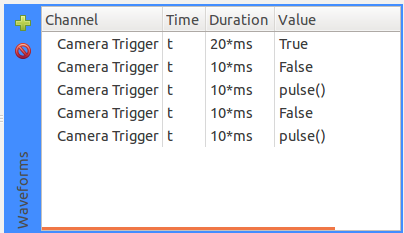
\includegraphics[width=.5\textwidth]{figures/waveform-3}}
          \centerline{b)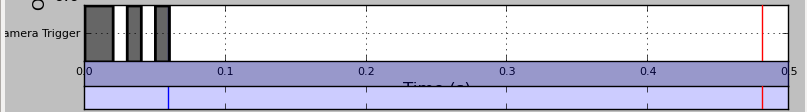
\includegraphics[width=.8\textwidth]{figures/plot-3}}
          \caption{a) Add some simple waveform elements. b) Plot of simple
          waveform elements.}
          \label{fig:quick:waveform-3}
        \end{figure}

        \begin{figure}[ht]
          \centerline{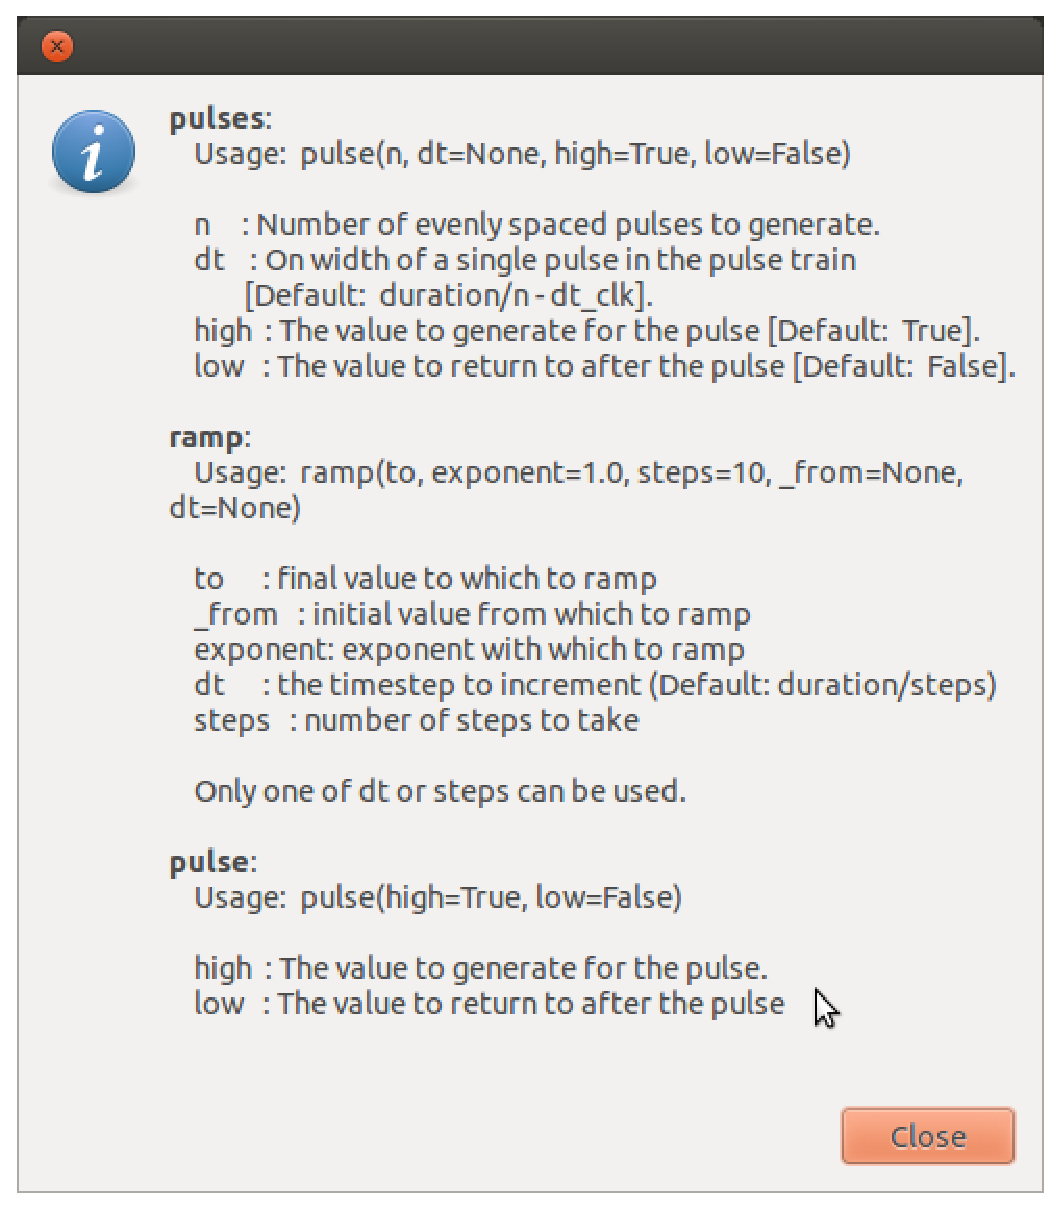
\includegraphics[width=.8\textwidth]{figures/generators}}
          \caption{Generators that can be used as element values.  These
          generators create multiple actual waveform transitions where the
          transition values and timing fit a prescribed functional form.}
          \label{fig:quick:generators}
        \end{figure}

        \begin{figure}[ht]
          \centerline{a)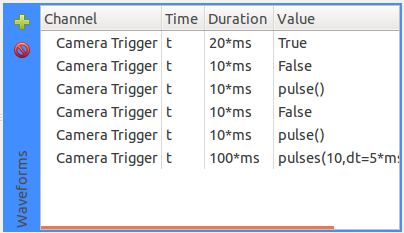
\includegraphics[width=.5\textwidth]{figures/waveform-4}}
          \centerline{b)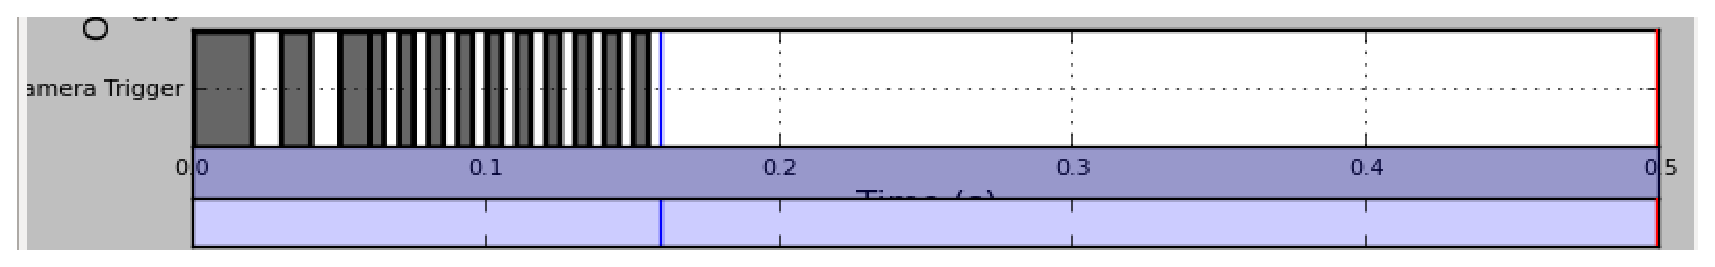
\includegraphics[width=.8\textwidth]{figures/plot-4}}
          \caption{a) Add some simple waveform elements. b) Plot of simple
          waveform elements.}
          \label{fig:quick:waveform-4}
        \end{figure}

        \begin{figure}[ht]
          \centerline{a)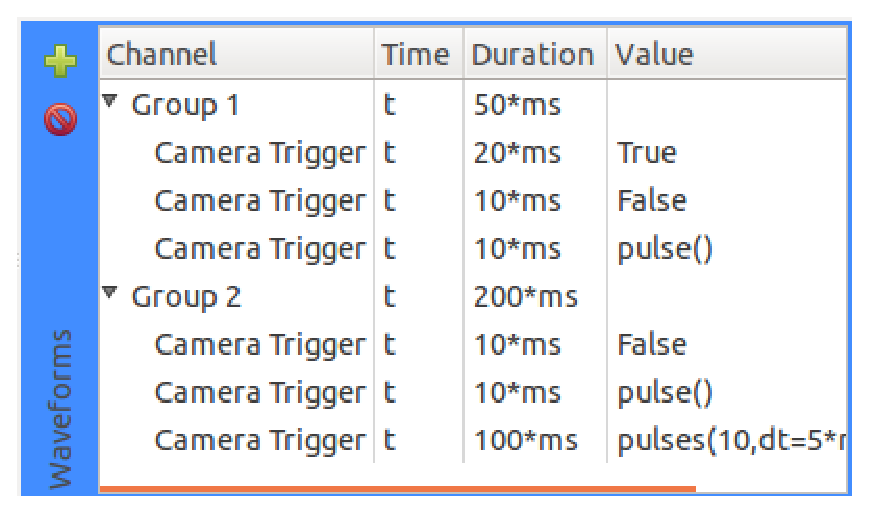
\includegraphics[width=.5\textwidth]{figures/waveform-5}}
          \centerline{b)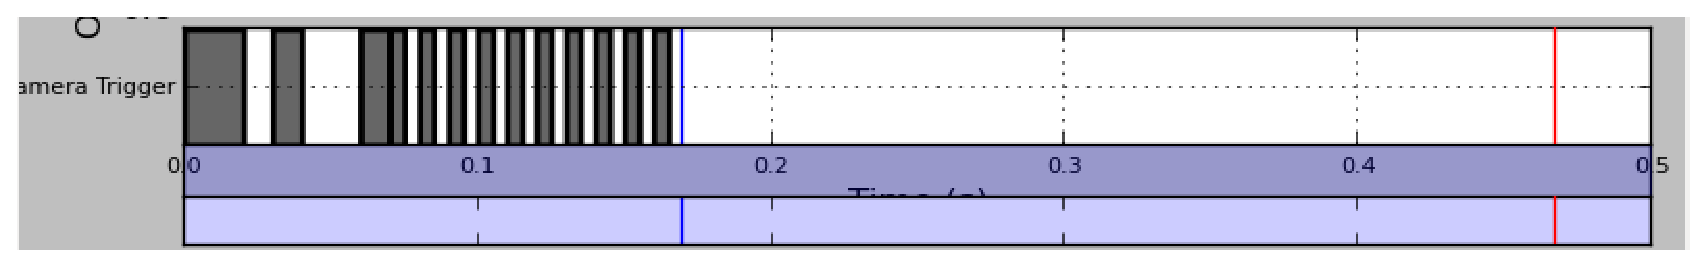
\includegraphics[width=.8\textwidth]{figures/plot-5}}
          \caption{a) Waveform elements divided into two main groups. b) Plot of
          waveform after grouping elements.}
          \label{fig:quick:waveform-5}
        \end{figure}

        \begin{figure}[ht]
          \centerline{a)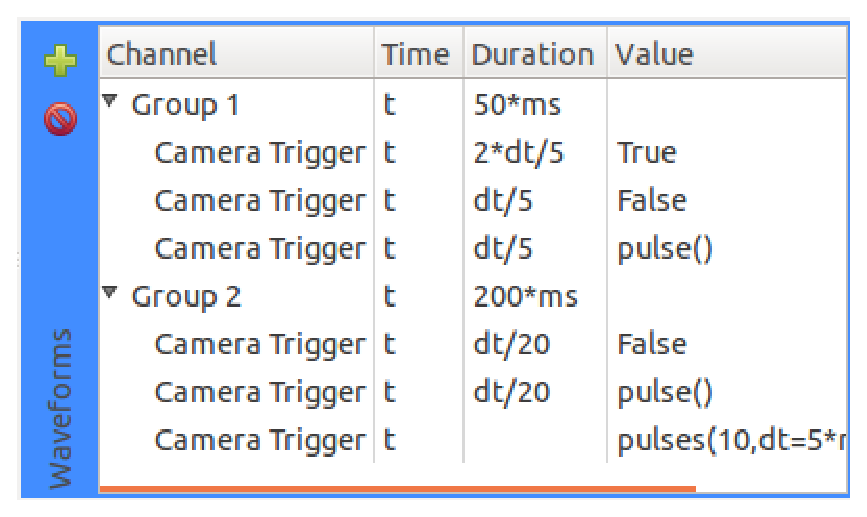
\includegraphics[width=.5\textwidth]{figures/waveform-6}}
          \centerline{b)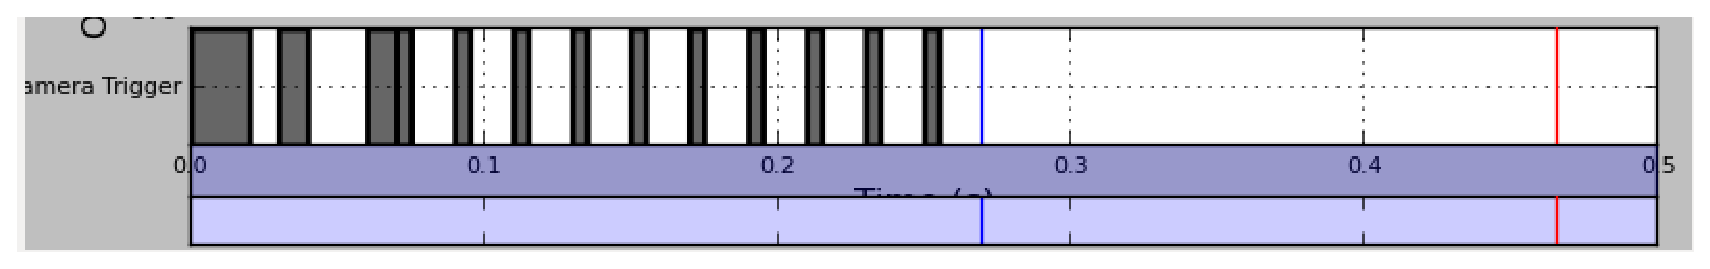
\includegraphics[width=.8\textwidth]{figures/plot-6}}
          \caption{a) Using automatic $dt$ variable. b) Plot of waveform after
          using $dt$ variable.}
          \label{fig:quick:waveform-6}
        \end{figure}


    \end{enumerate}
  \item Execute Waveform
\end{enumerate}
